\documentclass[a4paper]{article}
\usepackage[a4paper,  margin=1.0in]{geometry}

\usepackage{graphicx}
\usepackage{float}
\usepackage{hyperref}
\usepackage{listings}
\lstset{
basicstyle=\small\ttfamily,
columns=flexible,
breaklines=true
}

\usepackage{polski}
\usepackage[utf8]{inputenc}
\begin{document}


\title{Ćwiczenie nr 3 z MBI, Resekwencjonowanie genomu człowieka}
\author{Mateusz Chydziński, Michał Sypetkowski}
\maketitle

\section{Ogólne informacje}
Repozytorium git: \url{https://github.com/msypetkowski/MBI-exercises.git}.
W katalogu \texttt{cw3} repozytorim zawiera skrypty/polecenia użyte do przeprowadzenia eksperymentów.

\section{Mapowanie}

Najpierw indeksujemy plik FASTA (w pliku jest jedna sekwencja) genomu referencyjnego człowieka --
u nas tylko chromosom 1.

Następnie generujemy plik SAM (Sequence Alignment Map) za pomocą algorytmu bwa mem.
Plik ten zawiera zbiór mapowań sekwencji na (ang. aligned to) do sekwencji referencyjnej.
W naszym przypadku sekwencja referencyjna to plik chr1.fa,
a na tą sekwencę mapujemy sekwencje (odczyty z sekwencera)
z pliku coriell\_chr1.fq (zawiera on około 284k sekwencji).
Plik SAM zawiera mapowania kolejnych sekwencji z pliku coriell\_chr1.fg.

Następnie sortujemy te mapowania (mapowanie zawiera przy okazji sekwencje)
i tworzymy ich binarną reprezentację (plik BAM).
Stąd plik SAM ma 73MB, a BAM 14MB (mniej).

Plik FASTQ zawiera sekwencje (odczyty) i "quality value characters"
dla każdej sekwencji równe jej długości.
Plik SAM również zawiera sekwencje (tyle samo i takiej samej długości co FASTQ - 
ale są to dopasowane sekwencje z genomu referencyjnego a nie z odczytów)
i analogicznie odpowiadające "quality value characters".
Plik FASTQ ze ma rozmiar 55M --
mniej niż SAM, bo nie zawiera informacji o mapowaniu na genom referencyjny.

Średnia długość sekwencji odczytu to 75.5 z odchyleniem standardowym 1.17.

\section{Wizualizacja w IGV oraz przykładowy wariant w genie IQGAP3}  

Pozycja przykładowego wariantu to 156,496,188.
Referencyjny genom zawiera nukleotyd A a odczyty wskazują G.
81 odczytów wskazuje na wariant i żaden na referencje.
Zrzut ekranu z IGV jest na rysunku \ref{fig:igv}.
% TODO: homo czy heterozygota ?

\begin{figure}[h]
    \centering
    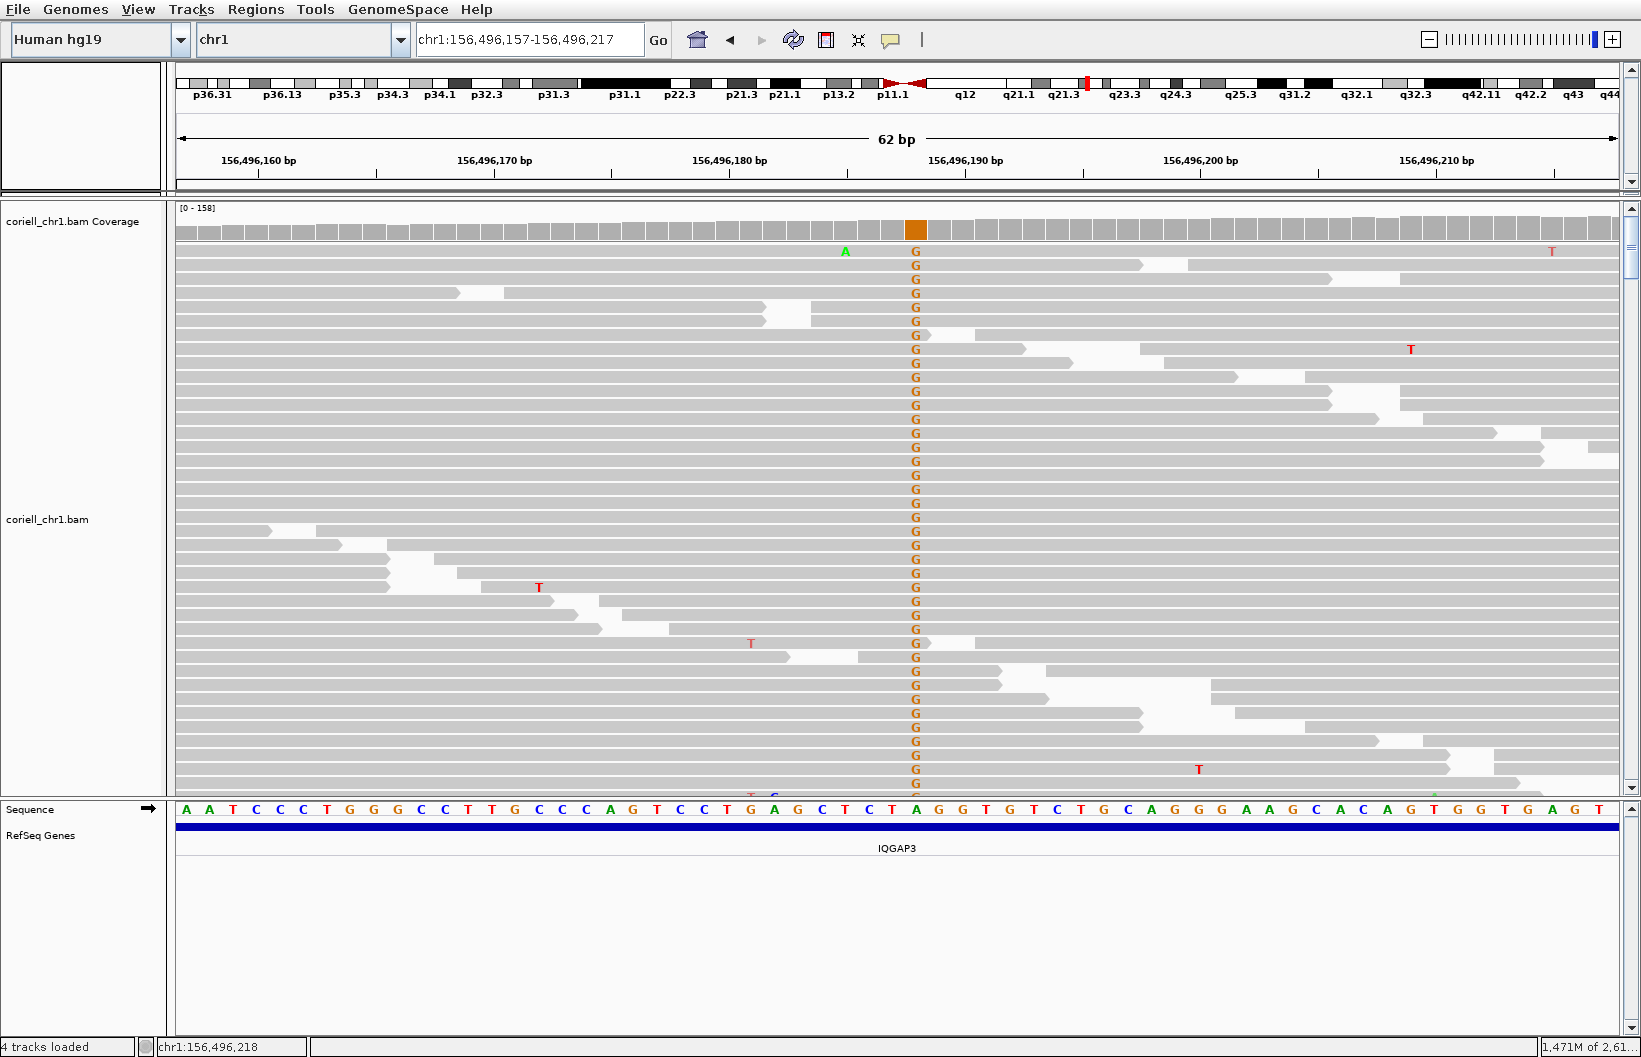
\includegraphics[width=1.0\textwidth]{sampleVariant.png}
    \label{fig:igv}
    \caption[]{Przykładowy wariant w oknie IGV}
\end{figure}


\section{Wykrywanie wariantów}  

Ilość wariantów bez filtracji to 6050, po filtracji -- 241.
% TODO

\section{Adnotacje wariantów}  
Po przeanalizowaniu pliku VCF narzędziem Variant Effect Predictor otrzymano wykres kołowy wariantów, na którym dominujący jest intron\_variant: 36\%.
Wiersze odpowiadające temu wariantowi:
\begin{verbatim}
.	1:156496188-156496188	G	3_prime_UTR_variant	MODIFIER	IQGAP3	ENSG00000183856	Transcript	ENST00000361170	protein_coding	38/38	-	-	-	4997	-	-	-	-	rs6427315	-	-1	-	HGNC	20669	-	-	-	-	0.9383	0.7746	0.9841	1	1	1	-	-	-	-	-	-	-	-	-	-	-	-	-	-	-	-	-	-	-
.	1:156496188-156496188	G	upstream_gene_variant	MODIFIER	snoU13	ENSG00000238843	Transcript	ENST00000458777	snoRNA	-	-	-	-	-	-	-	-	-	rs6427315	2934	1	-	RFAM	-	-	-	-	-	0.9383	0.7746	0.9841	1	1	1	-	-	-	-	-	-	-	-	-	-	-	-	-	-	-	-	-	-	-
.	1:156496188-156496188	G	3_prime_UTR_variant,NMD_transcript_variant	MODIFIER	IQGAP3	ENSG00000183856	Transcript	ENST00000491900	nonsense_mediated_decay	37/38	-	-	-	4973	-	-	-	-	rs6427315	-	-1	-	HGNC	20669	-	-	-	-	0.9383	0.7746	0.9841	1	1	1	-	-	-	-	-	-	-	-	-	-	-	-	-	-	-	-	-	-	-
\end{verbatim}
Jest to wariant w sekwencji kodującej (świadczy o tym wartość protein\_coding w kolumnie Exon) w pierwszym wierszu powyższego listingu.
\section{Wnioski}
Ćwiczenie polegało na analizie danych pozyskanych w trakcie resekwencjonowania fragmentu genomu człowieka. Przedmiotem badań był fragment sekwencji, dotyczący chromosomu pierwszego (chr1). Mapowanie danej sekwencji do sekwencji referencyjnej dostarczyło nam dodatkowych danych w postaci wykrytych wariantów. Dane z pliku SAM w sposób czytelny dla człowieka wizualizuje narzędzie IGV. Pozwala ono na sprawdzenie nie tylko faktu różnic w stosunku do genomu referencyjnego, ale także zmierzenie tej różnicy (liczba oznaczonych nukleotydów innych niż referencyjne, zsumowana dla wszystkich pokryć). Raport wygenerowany z filtrowanego pliku VCF poprzez narzędzie Variant Effect Predictor pozwolił dowiedzieć się o typie adnotowanych wariantów. Wiele z nich występuje w sekwencjach niekodujących - intronach (36\%) oraz transkryptach niekodujących (10\%). Spośród części kodujących, najwięcej jest wariantów synonimicznych (57\%), czyli takich, które kodują ten sam aminokwas. Jest to możliwe dlatego, że DNA jest "zdegenerowane", to znaczy istnieje kilka sekwencji (kodonów), które kodują ten sam aminokwas.
\end{document}
